\documentclass[10pt,landscape]{article}
\usepackage[ngerman]{babel}
\usepackage{multicol}
\usepackage{calc}
\usepackage{ifthen}
\usepackage[landscape]{geometry}
\usepackage{amsmath,amsthm,amsfonts,amssymb}
\usepackage{color,graphicx,overpic}
\usepackage{hyperref}
\usepackage{listings}
\usepackage[compact]{titlesec} %less space for headers
\usepackage{mdwlist} %less space for lists

\pdfinfo{
    /Title (Rechnerarchitekturen 2 -- Cheatsheet)
    /Creator (TeX)
    /Producer (pdfTeX 1.40.0)
    /Author (Robert Jeutter)
    /Subject ()
}

% This sets page margins to .5 inch if using letter paper, and to 1cm
% if using A4 paper. (This probably isn't strictly necessary.)
% If using another size paper, use default 1cm margins.
\ifthenelse{\lengthtest { \paperwidth = 11in}}
    { \geometry{top=.5in,left=.5in,right=.5in,bottom=.5in} }
    {\ifthenelse{ \lengthtest{ \paperwidth = 297mm}}
        {\geometry{top=1cm,left=1cm,right=1cm,bottom=1cm} }
        {\geometry{top=1cm,left=1cm,right=1cm,bottom=1cm} }
    }

% Turn off header and footer
\pagestyle{empty}

% Redefine section commands to use less space
\makeatletter
\renewcommand{\section}{\@startsection{section}{1}{0mm}%
                                {-1ex plus -.5ex minus -.2ex}%
                                {0.5ex plus .2ex}%x
                                {\normalfont\large\bfseries}}
\renewcommand{\subsection}{\@startsection{subsection}{2}{0mm}%
                                {-1explus -.5ex minus -.2ex}%
                                {0.5ex plus .2ex}%
                                {\normalfont\normalsize\bfseries}}
\renewcommand{\subsubsection}{\@startsection{subsubsection}{3}{0mm}%
                                {-1ex plus -.5ex minus -.2ex}%
                                {1ex plus .2ex}%
                                {\normalfont\small\bfseries}}
\makeatother

% Define BibTeX command
\def\BibTeX{{\rm B\kern-.05em{\sc i\kern-.025em b}\kern-.08em
    T\kern-.1667em\lower.7ex\hbox{E}\kern-.125emX}}

% Don't print section numbers
\setcounter{secnumdepth}{0}

\setlength{\parindent}{0pt}
\setlength{\parskip}{0pt plus 0.5ex}    
% compress space
\setlength\abovedisplayskip{0pt}
\setlength{\parskip}{0pt}
\setlength{\parsep}{0pt}
\setlength{\topskip}{0pt}
\setlength{\topsep}{0pt}
\setlength{\partopsep}{0pt}
\linespread{0.5}
\titlespacing{\section}{0pt}{*0}{*0}
\titlespacing{\subsection}{0pt}{*0}{*0}
\titlespacing{\subsubsection}{0pt}{*0}{*0}

%My Environments
\newtheorem{example}[section]{Example}
% -----------------------------------------------------------------------

\begin{document}


\begin{multicols}{2}
\footnotesize
\begin{description}
  \item[Ausführungszeit] $t[s]=\frac{\text{Taktzyklen [Takte]}}{\text{Frequenz [Hz]}} =\frac{C}{f}$
  \item[Leistung absolut] $L_{abs}[MIPS]=\frac{\text{Befehlsanzahl}}{\text{Ausführungszeit [s]}*10^6}=\frac{n}{t*10^6}$
  \item[Leistung relativ] $L_{rel}[MIPS]=\frac{\text{Referenzzeit [s]}}{\text{Ausführungszeit [s]}}*\text{RefLeistung [MIPS]} = \frac{t_{ref}}{t_mess}*L_{ref}$
  \item[Clocks per Instruction] $CPI=\frac{\text{Taktzyklen [Takte]}}{\text{Befehlsanzahl}} =\frac{C}{n}$
  \item[Gewichtete mittlere CPI] $CPI_{G}=\sum (CPI_{Befehlsgruppe}*\text{RelativeHäufigkeit}_{Befehlsgruppe})=\sum_{i=1}^n(CPI_i*p_i)$
  \item[Instructions per Clock] $IPC=\frac{Befehlsanzahl}{\text{Taktzyklen [Takt]}}=\frac{n}{C}$
  \item[Speedup] $S_n=\frac{1}{AnteilSeriell + Overhead + \frac{AnteilParallel}{AnzahlProzessoren}}=\frac{1}{ A_{seriell} + o(n) + \frac{ A_{parallel} }{ n }}$
  \item[Effizienz] $E_n=\frac{Speedup}{AnzahlProzessoren}=\frac{S_n}{n}$
\end{description}
\end{multicols}

\raggedright
\footnotesize
\begin{multicols}{3}
  
  % multicol parameters
  % These lengths are set only within the two main columns
  \setlength{\columnseprule}{0.25pt}
  \setlength{\premulticols}{1pt}
  \setlength{\postmulticols}{1pt}
  \setlength{\multicolsep}{1pt}
  \setlength{\columnsep}{2pt}

  \paragraph{CISC}
  \begin{itemize*}
    \item Complex Instruction Set Computing
    \item Einfache und komplexe Befehle
    \item Heterogener Befehlssatz
    \item Verschiedene Taktzahl pro Befehl
    \item Viele Befehlscode-Formate mit unterschiedlicher Länge
    \item Mikroprogrammwerk                             
    \item Vermischung von Verarbeitungs \& Speicherbefehlen
    \item schwierig, unter CPI = 2 zu kommen
  \end{itemize*}
  
  \paragraph{RISC}
  \begin{itemize*}
    \item Reduced Instruction Set Computing
    \item wenige, einfache Befehle
    \item Orthogonaler Befehlssatz   
    \item Meist 1 Takt pro Befehl
    \item Wenige Befehlscode-Formate mit einheitlicher Länge 
    \item Direktverdrahtung
    \item Trennung von Verarbeitungs \& Speicherbefehlen  
    \item Hohe Ausführungsgeschwindigkeit $(CPI \leq 1)$
  \end{itemize*}
  
  \paragraph{MIPS}
  \begin{itemize*}
    \item Microprocessor without interlocked pipeline stages
    \item 32-bit Architektur/64-bit Erweiterung
  \end{itemize*}
  
  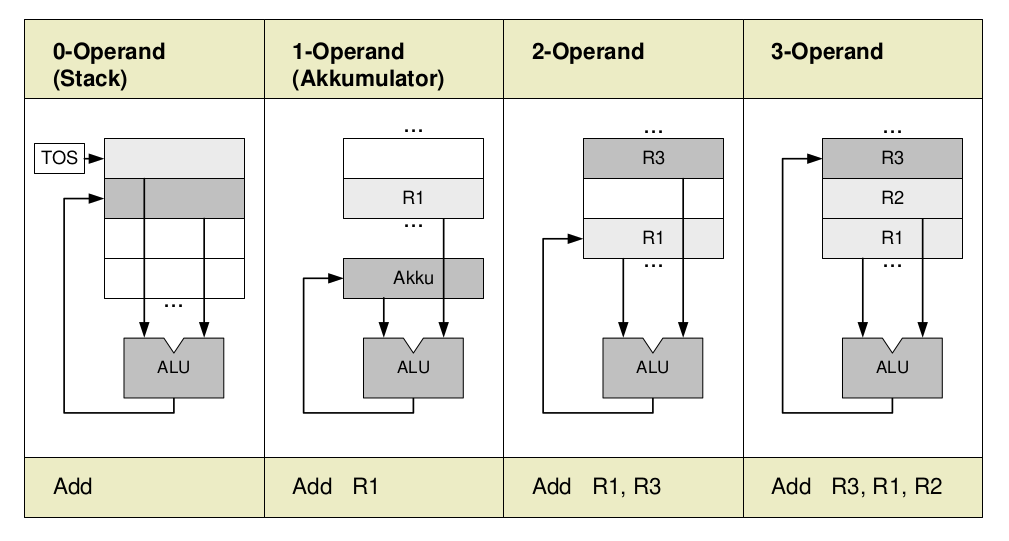
\includegraphics[width=\textwidth/4]{Assets/RA2_Operanden.png}
  
  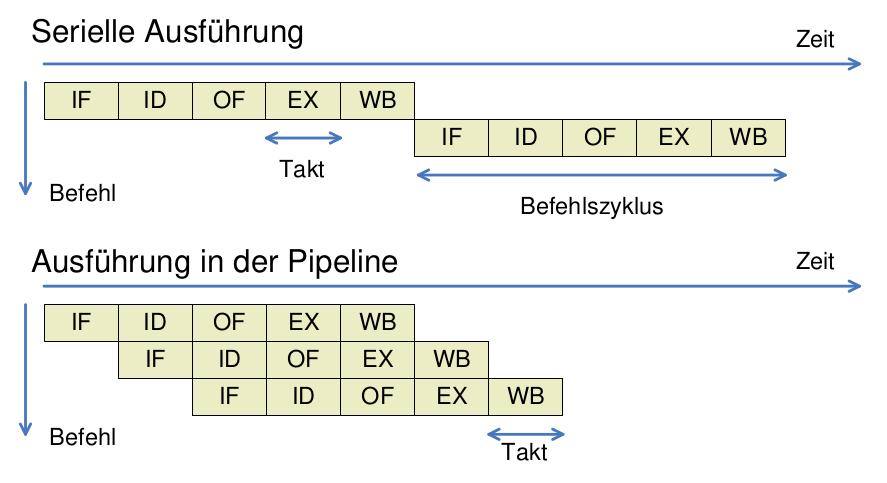
\includegraphics[width=\textwidth/4]{Assets/RA2_pipelineCPU.png}
  
  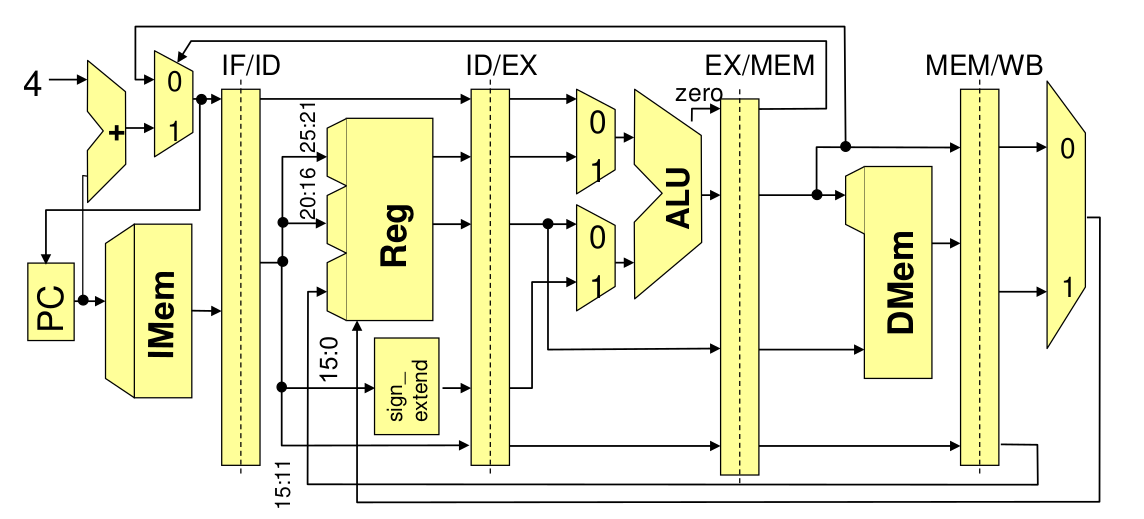
\includegraphics[width=\textwidth/4]{Assets/RA2_mehrzyklenCPU.png}
  
  Aufgaben der einzelnen Phasen
  \begin{description}
    \item[Befehlsholphase] Lesen des aktuellen Befehls; separater Speicher, zur Vermeidung von Konflikten mit Datenzugriffen
    \item[Dekodier \& Register-Lese-Phase] Lesen der Register möglich wegen fester Plätze für Nr. im Befehlswort
    \item[Ausführungs \& Adressberechnungsphase] Berechnung arithmetischer Funktion bzw. Adresse für Speicherzugriff
    \item[Speicherzugriffsphase] Wird nur bei Lade \& Speicherbefehlen benötigt
    \item[Abspeicherungsphase] Speichern in Register, bei Speicherbefehlen nicht benötigt
  \end{description}
  
  \paragraph*{Hazards}
  \begin{itemize*}
    \item resource hazards
    \item data hazards: Datenabhängigkeiten
    \begin{description}
      \item[Antidatenabhängig] falls Befehl j eine Speicherzelle beschreibt, die von i noch gelesen werden müsste. WAR (write after read)
      \item[Ausgabeabhängig] falls Befehle i und j die selbe Speicherzelle beschreiben. WAW (write after write)
      \item[Datenabhängigkeit] Operation hängt von der vorhergehenden Operation ab. RAW (read after write)
    \end{description}
    \item control hazards: Kontrollabhängigkeiten
    \begin{itemize*}
      \item Gleichheit der Register wird schon in der instruction decode-Stufe geprüft
      \item Sprungziel wird in separatem Adressaddierer ebenfalls bereits in der instruction decode-Stufe berechnet
    \end{itemize*}
  \end{itemize*}
  
  \subsection{ Sprungvorhersage}
  \paragraph{Einfache lokale Prädiktoren}
  \begin{itemize*}
    \item Liefern Vorhersage, ob bedingter Sprung genommen wird oder nicht
    \item Prädiktion allein anhand der Historie des betrachteten, aktuellen Sprungs
    \item Historie eines Sprungs wird mit 1, 2 oder n Bits gepuffert
  \end{itemize*}
  
  \paragraph{ Einfache Sprungvorhersage (1 Bit)}
  \begin{itemize*}
    \item Sprungvorhersage-Puffer
    \item Branch prediction buffer oder branch history table
    \item Kleiner Speicher, der mit (Teil der) Adresse des Sprungbefehls indiziert wird
    \item Verwendet nur wenige untere Bits der Adresse
    \item Enthält 1 Bit: Sprung beim letzten Mal ausgeführt (taken) oder nicht (not taken)
    \item Prädiktion: Sprung verhält sich wie beim letzten Mal
    \item Nachfolgebefehle ab vorhergesagter Adresse holen
    \item Falls Prädiktion fehlerhaft: Prädiktionsbit invertieren
    \item Alle Sprünge, deren Adressen im Indexteil übereinstimmen, werden derselben Zelle im branch prediction buffer zugeordnet.
    \item Einfachste Art von Puffer (keine Tags, d.h. keine Überprüfung, ob Adresse tatsächlich im Puffer)
    \item Entspricht sehr einfachem Cache
    \item Hat eine bestimmte Kapazität
    \item Kann nicht für alle Sprünge (aktuelle) Einträge enthalten
    \item Reduziert branch penalty nur, wenn branch delay länger als Berechnung der Zieladresse mit branch prediction buffer dauert
    \item Prädiktion kann fehlerhaft sein
    \item Prädiktion kann von anderem Sprungbefehl stammen (mit gleichen Bits im Indexteil der Adressen)
  \end{itemize*}
  
  \paragraph{ Einführung von Tag Bits}
  \begin{itemize*}
    \item Nachteile des einfachen 1-Bit Vorhersageschemas
    \item Höhere Fehlerrate als überhaupt möglich, wenn Häufigkeit der Sprungentscheidungen betrachtet wird
    \item D.h. auch wenn Sprung fast immer ausgeführt (taken) wird, entstehen 2 Fehler anstatt 1
    \item Tag beseitigt eines der Probleme: gültiger Eintrag, falls Tag-Bits gleich sind
    \item Alle Sprünge, deren Adressen im Indexteil übereinstimmen, werden derselben Zelle im branch prediction buffer zugeordnet. Überprüfung mittels tags, ob es der richtige Eintrag ist.
    \item Allgemein: Fehlerrate von 1-Bit Prädiktor ist für Sprünge in Schleifenkonstrukten doppelt so hoch wie die Anzahl ausgeführter Sprünge
  \end{itemize*}
  
  \paragraph{ 2 Bit Vorhersagen}
  \begin{itemize*}
    \item Änderung der Vorhersage nur, wenn 2 falsche Vorhersagen in Folge
    \item 2-Bit Branch-Prediction Buffer: Speicherung der Historie, Befehlsadressen als Zugriffsschlüssel
  \end{itemize*}
  
  % !{Sprungvorhersage; Quelle RA2 Vorlesung 2020/21](Assets/RA2_Sprungvorhersage.png)
  
  \paragraph{ n-Bit Prädikator}
  Allgemein: n-Bit Prädiktor (Spezialfall: 2-Bit)
  \begin{itemize*}
    \item Verwendet n-Bit Zähler
    \item Sättigungsarithmetik (kein wrap around bei Überlauf)
    \item Kann Werte zwischen 0 und $2^{n-1}$ annehmen
    \item Wenn Zähler größer als Hälfte des Maximums $(2^{n-1})$: Vorhersagen, dass Sprung ausgeführt wird; ansonsten vorhersagen, dass Sprung nicht genommen wird
    \item Zähler wird bei ausgeführtem Sprung inkrementiert und bei nicht ausgeführtem dekrementiert
    \item In der Praxis: 2-Bit Prädiktor ähnlich gut wie n-Bit Prädiktor
    \item In den meisten Prozessoren heute: 2-Bit Prädiktor für (lokale) Vorhersage
  \end{itemize*}
  
  \paragraph{ Korrelierende Prädikatoren}
  \begin{itemize*}
    \item Einschränkung des n-Bit (bzw. 2-Bit) Prädiktors:
    \item Betrachtet nur (vergangenes) Verhalten eines Sprungs, um dessen (zukünftiges) Verhalten vorherzusagen.
    \item Arbeitet rein lokal!
    \item Idee: Verbesserung durch Betrachtung des Verhaltens anderer Sprünge
    \item Man erhält so genannten korrelierenden Prädiktor (correlating predictor) oder zweistufigen Prädiktor
    \item Prinzip: Aufgrund globaler Information (anderer Sprünge) wird einer von mehreren lokalen Prädiktoren ausgewählt
    \item Beziehen zur Vorhersage des Verhaltens eines Sprungs Kontext-Information mit ein, d.h. die Historie anderer Sprungbefehle
    \item Prädiktor benutzt globale Kontext-Bits, um einen von mehreren lokalen Prädiktoren auszuwählen
    \item Betrachten wiederholte Ausführung des Codefragments (ignorieren dabei alle anderen Sprünge, inkl. dem für Wiederholung)
  \end{itemize*}
  
  Zweistufiger Prädiktor
  \begin{itemize*}
    \item Verwendet 1 Bit Kontextinformation
    \item Es existieren 2 lokale Prädiktoren, beide je 1-Bit
    \item Kontext: Letzter (i.a. anderer) Sprung wurde ausgeführt/nicht ausgeführt (1 Bit)
    \item Vorhersage des zweistufigen Prädiktors: Anhand des Kontexts wird lokaler Prädiktor für die Vorhersage des aktuell betrachteten Sprungs ausgewählt
    \item Letzter Sprung ist i.a. nicht gleich aktuellem, vorherzusagendem Sprung (nur in einfachen Schleifen)
    \item Notation des Prädiktorstatus: `<X>/<Y>` mit
    \item `<X>`: Vorhersage, falls letzter Sprung not taken, d.h. Kontext = NT
    \item `<Y>`: Vorhersage, falls letzter Sprung taken, d.h. Kontext = T
    \item `<X>` und `<Y>` Vorhersagen: jeweils entweder T oder NT
  \end{itemize*}
  
  (m,n)-Prädiktor
  \begin{itemize*}
    \item Betrachtet als Kontext das Verhalten der letzten m Sprünge, um aus $2^m$ vielen lokalen Prädiktoren einen n-Bit Prädiktor auszuwählen
    \item Vorteil gegenüber (rein lokalem) 2-Bit Prädiktor
    \item Höhere Vorhersagegenauigkeit
    \item Erfordert kaum Hardwareaufwand
    \item Sprunggeschichte (Kontext, „Ausgang“ vorangegangener Sprünge) kann in m-Bit Schieberegister gespeichert werden (1 Bit für jeden der m vielen letzten Sprünge im Kontext, Bit gleich 1 wenn Sprung taken)
    \item Vorhersagepuffer adressiert via Konkatenation von
    \item Unteren Adressbits der Sprungbefehlsadresse
    \item m Bit globaler Sprunggeschichte
  \end{itemize*}
  
  \paragraph{ High Performance Befehlsdekodierung}
  In Hochleistungs-Pipelines ist reine Vorhersage eines Sprungs i.d.R. nicht ausreichend
  \begin{itemize*}
    \item Insbesondere: Falls mehrere Befehle pro Takt auszugeben sind
    \item Befehlsstrom mit großer Bandbreite erforderlich!
    \item Kontrollflussabhängigkeiten dürfen nicht „wahrnehmbar“ sein 
    \item Maßnahmen hierfür
    \item Pufferung von Sprungzielen, und nicht nur Vorhersage des Sprungverhaltens (branch target buffer)
    \item Integrierte Einheit für das Holen der Befehle (d.h. nicht nur [relativ] einfache erste Stufe der Pipeline)
    \item Vorhersage von Rücksprungadressen (bei Prozeduraufruf)
  \end{itemize*}
  
  \paragraph{ Branch Target Buffer}
  5-stufige Pipeline, Auswertung von Sprungbedingungen in EX:
  \begin{itemize*}
    \item Branch delay von 2 Takten
    \item Mit Sprungvorhersage (branch prediction buffer)
    \item Zugriff erfolgt in ID (Adresse des Sprungbefehls schon in IF bekannt; aber:
    \item evtl. angesprungenes Ziel erst nach Befehlsdecodierung [ID])
    \item Nächste vorhergesagte Instruktion kann erst nach ID geholt werden
    \item Branch delay = 1, falls Prädiktion korrekt
    \item Mit Pufferung des Sprungziels (branch target buffer)
    \item Zugriff auf branch target buffer erfolgt in IF. Verhalten wie „echter“ Cache,
    \item adressiert mit Sprungbefehlsadresse (überprüft, ob Cache-Hit)
    \item Liefert vorhergesagte Adresse als Ergebnis, d.h. nächsten PC (d.h. nicht nur Vorhersage über Sprungverhalten)
    \item Keine Verzögerung, falls Prädiktion korrekt!
  \end{itemize*}
  
  Zusätzliche Speicherung auch des Sprungziels, z.B. Kombination mit branch prediction buffer
  
  Bei geschickter Organisation kann das Fließband immer gefüllt bleiben; die Sprünge kosten dann effektiv keine Zeit; CPI <1 möglich.
  
  Eigenschaften
  \begin{itemize*}
    \item Verzögerung durch Sprung kann vollständig vermieden werden (sofern Vorhersage korrekt), da bereits in IF Entscheidung über nächsten Befehlszähler (PC) getroffen wird.
    \item Da Entscheidung allein auf Basis des PC getroffen wird, muss überprüft werden, ob Adresse im Puffer (impliziert, dass Sprungbefehl vorliegt)
    \item Speicherung im Prinzip nur für Sprünge notwendig, die als ausgeführt vorhergesagt werden (not taken = normale sequentielle Dekodierung geht weiter)
    \item Achtung – bei falscher Vorhersage
    \item Entsteht ursprüngliche Sprung-Verzögerung, plus
    \item Aufwand zur Aktualisierung des Vorhersagepuffers
  \end{itemize*}
  
  \paragraph{ Integrierte Befehls-Hol-Einheit (IF Unit)}
  Insbesondere mit Blick auf multiple-issue Prozessoren eigene (autonome) funktionale Einheit für Befehlsholphase
  \begin{itemize*}
    \item Führt Befehlscodes in Pipeline ein
    \item Integrierte Funktionalitäten
    \item Sprungvorhersage: Wird Teil der Befehlsholphase
    \item Instruction Pre-fetch: Insbes. um mehrere Befehle pro Takt liefern (und später ausgeben) zu können, läuft Befehlsholen weiterer Dekodierung voraus (= pre-fetch)
    \item Zugriff auf Befehlsspeicher: Bei mehreren Befehlen pro Takt mehrere Zugriffe erforderlich (bei Cache auf ggfs. mehrere cache lines). Werden hier koordiniert/geplant
    \item Befehlspuffer: Befehle können hier (lokal im Prozessor!) von Issue-Stufe nach Bedarf abgerufen werden
  \end{itemize*}
  
  \paragraph{ Vorhersage von Rücksprungadressen}
  Allgemeines Ziel: Vorhersage indirekter Sprünge (d.h. bzgl. Basisadresse in Register)
  \begin{itemize*}
    \item Hauptverwendung: Rückkehr aus Prozeduraufrufen
    \item MIPS: Prozeduraufruf per jal proc, Rückkehr per jr \$31
    \item Vorhersage mit branch target buffer schlecht, da Aufruf aus unterschiedlichen Codeteilen heraus möglich
    \item Methode: (Stack-) Speicher für Rücksprungadressen
    \item Push bei Prozeduraufruf (call), und
    \item Pop bei Rücksprung (return)
    \item Vorhersagequalität „perfekt“, wenn Stack-Puffer größer als maximale Aufruftiefe
  \end{itemize*}
  
  
  \section{ Multiple-Issue-Architekturen}
  \subsection{ Mehrere Ausführungseinheiten}
  \begin{itemize*}
    \item Techniken der vorangegangenen Abschnitte geeignet, um Daten- und Kontrollkonflikte zu lösen
    \item Idealer CPI ~1
    \item Weitere Leistungssteigerung: 
    \item CPI < 1
    \item Mehrere Befehle pro Takt ausgeben (fertigstellen)
    \item Zwei Grundtypen von multiple-issue Prozessoren:
    \item Superskalar
    \item Geben variable Anzahl von Befehlen pro Takt aus
    \item Mit statischem (vom Compiler erzeugtem) oder dynamischem Scheduling in Hardware
    \item VLIW/EPIC
    \item Feste Anzahl von Befehlen ausgegeben, definiert durch Befehlscode (weitgehende Planung der Issue-Phase durch Compiler)
  \end{itemize*}
  
  % !{In Order Pipeline; Quelle RA2 Vorlesung 2020/21](Assets/RA2_in-order-pipeline.png)
  
  \subsection{ Superskalar}
  statisch: Details der Befehlsausgabe
  \begin{itemize*}
    \item In IF werden 1-n Befehle von Instruction Fetch Unit geholt (ggfs. Max. von n nicht immer möglich, z.B. bei Sprüngen)
    \item Befehlsgruppe, die potentiell ausgegeben werden kann = issue packet
    \item Konflikte bzgl. Befehlen im issue packet werden in Issue-Stufe in Programmreihenfolge (d.h. in-order) geprüft
    \item Befehl ggfs. nicht ausgegeben (und alle weiteren)
    \item Aufwand für Prüfung in Issue-Stufe groß!
    \item Wegen Ausgewogenheit der Pipeline-Stufen ggfs. Issue weiter „pipelinen“, d.h. in mehrere Stufen unterteilen = nicht-trivial
    \item Parallele Ausgabe von Befehlen limitierender Faktor superskalarer Prozessoren!
  \end{itemize*}
  
  MIPS mit statischem Scheduling
  \begin{itemize*}
    \item Annahme: 2 Befehle pro Takt können ausgegeben werden (1x ALU, Load/Store plus 1x FP)
    \item Einfacher als 2 beliebige Befehle (wegen „Entflechtung“)
    \item Befehlsstart umfasst
    \item 2 Befehlsworte holen (64-Bit Zugriff, d.h. komplexer als bei nur 1 Befehl \item ggfs. Pre-fetch?)
    \item Prüfen, ob 0, 1 oder 2 Befehle ausgegeben werden können
    \item Befehl(e) ausgeben an korrespondierende funktionale Einheiten
    \item Prüfen auf Konflikte durch Entflechtung vereinfacht
    \item Integer und FP-Operationen nahezu unabhängig (verschiedene Registersätze)
    \item Abhängigkeiten nur bei Speichertransfers möglich (von Integer-ALU für FP ausgeführt) \item Einschränkung des issue 
    \item Leistungssteigerung nur bei „geeignetem“ Anteil von FP-Operationen im Programm sowie geeigneter „Verflechtung“ durch Compiler!
  \end{itemize*}
  
  \subsection{ Dynamisches Befehlsscheduling – in-order execution}
  Bislang
  \begin{itemize*}
    \item Reihenfolge der Befehlsabarbeitung = Reihenfolge der Befehle im Speicher, abgesehen von Sprüngen
    \item Behindert schnelle Ausführung
  \end{itemize*}
  
  Scoreboarding
  \begin{itemize*}
    \item Jeder Befehl, der aus der Instruction fetch-Einheit kommt, durchläuft das Scoreboard.
    \item Wenn für einen Befehl alle Daten/Operanden bekannt sind und die Ausführungseinheit frei ist, wird der Befehl gestartet.
    \item Alle Ausführungseinheiten melden abgeschlossene Berechnungen dem Scoreboard.
    \item Dieses erteilt Befehlen die Berechtigung zum Abspeichern von Ergebnissen, sofern
    \item Speichereinheit frei ist und
    \item Antidaten- und Ausgabeabhängigkeiten berücksichtigt sind und prüft, ob dadurch neue Befehle ausführbereit werd
    \item Zentrale Datenstruktur hierfür: Scoreboard (deutsch etwa „Anzeigetafel“ [für Befehlsstatus])
    \item Ursprünglich realisiert für CDC 6600 (1964):
    \item load/store-Architektur
    \item mehrere funktionale Einheiten (4xFP, 6xMem, 7xInteger ALU)
    \item Scoreboarding für MIPS nur sinnvoll
    \item für FP-Pipeline (Operationen mit mehreren Taktzyklen)
    \item und mehrere funktionale Einheiten (hier: 2 x Mult, Div, Add, Int)
  \end{itemize*}
  
  % !{Out Of Order Execution; Quelle RA2 Vorlesung 2020/21](Assets/RA2_out-of-order-execution.png)
  
  
  \paragraph{ Verfahren von Tomasulo}
  \begin{itemize*}
    \item Erdacht für IBM 360
    \item Verfahren von Tomasulo erlaubt auch bei Ausgabe- und Antidatenabhängigkeiten, die Reihenfolge zu vertauschen
    \item Umbenennung der Register; verschiedenen Benutzungen eines Registers werden verschiedene Speicherzellen zugeordnet
    \item Jeder funktionalen Einheit wird eine Reservation Station zugeordnet
    \item Reservation Stations enthalten die auszuführende Operation und, soweit bekannt, die Operanden bzw. eine Kennzeichnung in Form von tag bits des Operanden
    \item Sind alle Operanden bekannt und ist die funktionale Einheit frei, so kann die Bearbeitung beginnen
    \item Am Ende der Bearbeitung wird das Ergebnis von allen Einheiten übernommen, die das Ergebnis benötigen
    \item Verteilen der Daten erfolgt vor der Abspeicherung im Registerspeicher
    \item Aus den tag bits geht hervor, aus welcher Einheit der Operand kommen muss
    \item Registeradressen werden dynamisch auf größere Anzahl von Plätzen in den Reservation Stations abgebildet, d.h. Register effektiv umbenannt. Performance-Beschränkungen wegen weniger Register werden so umgangen
  \end{itemize*}
  
  \paragraph{ Register Renaming}
  \begin{itemize*}
    \item Prinzip: Verwendung temporärer Register für (logisch) neue möglicherweise interferierende Belegung
    \item Beispiel
    \item Annahme: es existieren zwei temporäre Register S und T
    \item Kollidierende Belegungen von F8 durch `sub.d` bzw. F6 durch `add.d` in (eindeutige) temporäre Register „umleiten“
    ```cpp
    div.d $F0,$F2,$F4
      add.d $T,$F0,$F8   // Lesen von F8, Schreiben von T (F6)
    s.d   $T,0($R1)    // Lesen von T (F6)
    sub.d S,$F10,$F14  // Schreiben von S (F8)
    mul.d $F6,$F10,S   // Schreiben von F6
    ```
    \item Alle Namenskonflikte durch Umbenennung auflösbar (Voraussetzung: genügend temporäre Register)
    \item Weitere Verwendung von F8/F6 durch S/T ersetzen!
    \item Wichtige Hardwarestruktur: Reservation Stations
    \item Zugeordnet zu funktionalen Einheiten (i.d.R. eine pro Einheit)
    \item Arbeitsweise von Reservation Stations
    \item Puffern Operanden für Befehle (sobald verfügbar/geladen)
    \item Müssen nicht aus Registern gelesen werden!
    \item Ausstehende Operanden verweisen auf Reservation Station, die Eingabe bereitstellen wird
    \item Bei aufeinander folgenden Schreibzugriffen auf Register: Nur letzter für Aktualisierung des Inhalts verwendet
    \item Wichtige Eigenschaften der Verwendung von Reservation Stations anstelle des zentralen Registersatzes
    \item Konfliktdetektion und Ausführungskontrolle verteilt
    \item Informationen in Reservation Stations bei den funktionalen Einheiten bestimmen, wann Ausführung eines Befehls möglich ist
    \item Ergebnisse werden direkt zu den funktionalen Einheiten (in jeweiliger Reservation Station) weitergereicht
    \item Erweiterte Form des Forwarding
    \item Realisiert implizit Register Renaming
    \item Möglich durch gemeinsamen Ergebnisbus (common data bus)
  \end{itemize*}
  
  
  \subsection{ Multiple-Issue mit dynamischem Scheduling}
  \begin{itemize*}
    \item Wesentlicher Nachteil von statischem Scheduling für superskalare Prozessoren: Latenzzeiten werden ca. mit Länge des issue packets skaliert
    \item „Längere“ Verzögerung (in Anzahl Befehlen) für Load/Stores bzw. Branches
    \item Lösung: Erweiterung des Tomasulo-Algorithmus auf Multiple-Issue durch
    \item Sequentielles Ausgeben mehrerer Befehle an Reservation Stations innerhalb eines Taktes, oder
    \item „Verbreiterung“ der Ausgabe-Logik (issue logic) zur Behandlung mehrerer Operationen parallel
    \item (alle Abhängigkeiten gleichzeitig überprüfen!)
  \end{itemize*}
  
  \paragraph{ VLIW - Very Long Instruction Word}
  VLIW (Very Long Instruction Word)-Prozessor
  \begin{itemize*}
    \item verschiedene parallele Ausführungseinheiten
    \item Verteilung von Maschinencode direkt vom Befehlswort im Speicher vorgegeben
    \item Sieht für jede Ausführungseinheit dezidierte Anweisungen vor
    \item keine Abhängigkeiten daher geringere Komplexität in Hardware
    \item Meist für stark parallelisierbare Aufgaben verwendet (Signalverarbeitung, Vektorrechner, DSP)
    \item Vorteile:
    \begin{itemize*}
      \item Die parallele Architektur des Prozessors kann schon während der der Programmerstellung (Kompilieren) zur Optimierung genutzt werden.
      \item Keine aufwendige Prozessorhardware zur Befehlsverteilung/Abhängigkeitsanalyse erforderlich (einfacherer Prozessor)
      \item Ausführungszeiten sind im wesentlichen bekannt
    \end{itemize*}
    \item Nachteile:
    \begin{itemize*}
      \item Aufwendigere Compiler
      \item Schlechte Prozessorauslastung bei ungünstigem Code
      \item Rekompilierung für den Prozessor erforderlich (kein Universalrechner)
      \item Größerer Speicherbedarf (Programm), wenn Code nicht parallelisiert werden kann.
    \end{itemize*}
  \end{itemize*}
  
  % !{VLIW Dynamisch; Quelle RA2 Vorlesung 2020/21](Assets/RA2_VLIW-dynamisch.png)
  
  EPIC = Explicitely Parallel Instruction Computing = IA64
  \begin{itemize*}
    \item Im wesentlichen Prinzip des VLIW-Prozessors
    \item Umsortieren der Befehle und Auflösung der Abhängigkeiten werden durch den Compiler durchgeführt
    \item Hauptnachteil; Neukompilierung erforderlich)
    \item Keine statische Aufteilung auf Funktionseinheiten
    \item Effizienteres Befehlswort \item Keine Verwendung von zwangsweise NOPs
  \end{itemize*}
  
  Bei der IA64-Architektur werden verschiedene Ansätze verfolgt, um die Prozessorlogik zu vereinfachen.
  \begin{enumerate*}
    \item Bedingte Befehlsverarbeitung
    \begin{itemize*}
      \item Ein Befehl wird abhängig von einem Statusbit ausgeführt
      \item Dadurch kann die Sprungvorhersage bei einfachen if-then-else Zweigen entfallen
      \item Die then und else Befehle sind parallel, wobei jeweils nur einer ausgeführt wird
    \end{itemize*}
    \item Statische Sprungvorhersage (Compiler)
    \item Die Optimierung (Finden paralleler Befehle) wird im wesentlichen dem Compiler überlassen.
    \item Spekulatives Laden von Operanden
    \begin{itemize*}
      \item Möglichst geringe Wartezeit auf Operanden
      \item Schon im Compiler werden entsprechende Ladebefehle vorgezogen.
    \end{itemize*}
  \end{enumerate*}
  
  % !{VLIW Vergleich; Quelle RA2 Vorlesung 2020/21](Assets/RA2_VLIW-vergleich.png)
  
  \subsection{ Simultaneous Multithreading (SMT)}
  % !{SMT; Quelle RA2 Vorlesung 2020/21](Assets/RA2_Simultaneous-Multithreading.png)
  
  \begin{itemize*}
    \item Modellprozessor I (2-fach Superskalar)
    \item Modellprozessor II (2-fach Out-of-Order)
  \end{itemize*}
  
  Ansätze zur Effizienzsteigerung durch Mikroparallelität
  | Bezeichnung | Konflikterkennung | Issue-Struktur | Scheduling | Hauptmerkmal | Beispiele |
  | -- | -- | -- | -- | -- | -- |
  | Superskalar (statisch) | Hardware | Dynamisch | Statisch | In-order Execution | Sun UltraSPARC II/ III |
  | Out of Order | Hardware | Dynamisch | Dynamisch mit Spekulation | Out of Order mit Spekulation | Pentium III, Pentium 4, MIPS 10000 | 
  | VLIW | Software | Statisch | Statisch | Keine Konflikte | Trimedia, diverse DSPs |
  
  \section{ Speicherarchitektur}
  \subsection{ Speicherhierarchie}
  \begin{itemize*}
    \item Große Speicher sind langsam
    \item Anwendung verhalten sich üblicherweise lokal
    \item Häufig benötigte Speicherinhalte in kleinen Speichern, seltener benötigte Inhalte in großen Speichern ablegen!
    \item Einführung einer „Speicherhierarchie“
    \item Illusion eines großen Speichers mit (durchschnittlich) kleinen Zugriffszeiten
    \item Bis zu sechs Ebenen in modernen Systemen unterscheidbar
  \end{itemize*}
  
  Ebene | Latenz | Kapazität 
  -- | -- | --
  Register | 100ps | 1 KByte
  Cache | 1ns | 12 MByte
  Hauptspeicher/RAM | 10ns | 8 GByte
  Festplatte | 10ms | 1 TByte
  CD-ROM/DVD/BlueRay | 100ms | 50 GByte
  Magnetbänder | 100s | 5 TByte
  
  \begin{itemize*}
    \item Adresspipelining
    % !{Pipelining; Quelle RA2 Vorlesung 2020/21](Assets/RA2_Adresspipelining.png)
    \item Matrixaufbau eines Speichers
    \item Aufteilen der Speicheradresse in Zeilen- und Spaltenadresse
    \item Lesezugriff auf Speicher
    \item Dekodierung der Zeilenadresse bestimmt Select-Leitung
    \item Komplette Zeile wird in den Zeilenpuffer geschrieben
    \item Durch Dekodierung der Spaltenadresse wird das gewünscht Datenwort ausgewählt
    \item Blocktransfer (Burst): Auslesen des kompletten Zeilenpuffers durch automatisches Inkrementieren der Spaltenadresse
  \end{itemize*}
  
  \subsection{ Typischer DRAM-Speicher}
  \begin{itemize*}
    \item Matrixaufbau eines DRAM-Speichers
    \item Adressleitungen werden i.d.R. gemultiplext
    \item Die gleichen Adressleitungen werden einmal zur Auswahl der Zeile verwendet, danach zur Auswahl der Spalte
    \item Einsparung von Leitungen, gerade für große Speicher wichtig
    \item Steuerleitungen RAS/CAS codieren, ob Adressleitungen Zeile oder Spalte auswählen
    \item RAS (Row Address Strobe): Bei einer fallenden Flanke auf RAS wird die anliegende Adresse als Zeilenadresse interpretiert
    \item CAS (Column Address Strobe): Bei einer fallenden Flanke auf CAS wird die anliegende Adresse als Spaltenadresse interpretiert
    \item Zugriff auf DRAM
    \item Erster Schritt
    \item Zeilenadressdecoder liefert Select-Leitung für eine Zeile
    \item Komplette Zeile wird in einen Zwischenpuffer übernommen
    \item Und zurückgeschrieben!
    \item Zweiter Schritt
    \item Aus dem Zwischenpuffer wird ein Wort ausgelesen
    \item Schritt kann mehrfach wiederholt werden (mehrere aufeinanderfolgende Wörter können gelesen werden)
    \item Auffrischung
    \item Heute auf dem DRAM-Speicher integriert
    \item Früher durch externe Bausteine ausgelöst
    \item DRAM-Eigenschaften
    \item Weniger Platzbedarf
    \item Nur 1 Transistor und 1 Kondensator pro Speicherzelle, statt 6 Transistoren bei SRAM
    \item Integrationsdichte Faktor 4 höher als bei SRAMs
    \item Langsamerer Zugriff
    \item Insbes. Lesezugriff wegen Zwischenspeicherung und Auffrischung
    \item Multiplexen der Adressleitungen
    \item Auf DRAM-Zeile kann während Auffrischung nicht zugegriffen werden
    \item Hoher Energieverbrauch sowohl bei Aktivität als auch bei Inaktivität
    \item Ausgleich des Ladungsverlusts durch periodische Auffrischung
    \item Zwischenpuffer und Logik zur Auffrischung
  \end{itemize*}
  
  Interleaving
  % !{Interleaving; Quelle RA2 Vorlesung 2020/21](Assets/RA2_Interleaving.png)
  
  \subsection{ Caches}
  \begin{itemize*}
    \item Cache = schneller Speicher, der vor einen größeren, langsamen Speicher geschaltet wird
    \item Im weiteren Sinn: Puffer zur Aufnahme häufig benötigter Daten
    \item Für Daten die schon mal gelesen wurden oder in der Nähe von diesen liegen
    \item 90% der Zeit verbringt ein Programm in 10% des Codes
    \item Im engeren Sinn: Puffer zwischen Hauptspeicher und Prozessor
    \item Ursprung: cacher (frz.) – verstecken („versteckter Speicher“)
    \item Organisation von Caches
    \item Prüfung anhand der Adresse, ob benötigte Daten im Cache vorhanden sind („Treffer“; cache hit)
    \item Falls nicht (cache miss): Zugriff auf den (Haupt-) Speicher, Eintrag in den Cache
    \item Prinzip eines Cache (Hit) % !{Cachehit; Quelle RA2 Vorlesung 2020/21](Assets/RA2_Cachehit.png)
    \item Cache-Strategien und Organisationen
    \item Wo kann ein Block im Cache abgelegt werden?
    \item Platzierung abhängig von der Organisationsform
    \item Organisationsform: direkt, mengenassoziativ, vollassoziativ
    \item Welcher Speicherblock sollte bei einem Fehlzugriff ersetzt werden?
    \item Ersetzungsstrategie: Zufällig, FIFO, LRU
    \item Was passiert beim Schreiben von Daten in den Cache?
    \item Schreibstrategie: write-back, write-through
    \item Direkt abgebildeter Cache
    \item Such-Einheit im Cache: Cache-Zeile (cache line).
    \item Weniger tag bits, als wenn man jedem Wort tag bits zuordnen würde.
    \item Cache-Blöcke, cache blocks
    \item Die Blockgröße ist die Anzahl der Worte, die im Fall eines cache misses aus dem Speicher nachgeladen werden.
    \item Beispiel: (Blockgröße = line size)
    \item Wenn block size < line size, dann sind zusätzliche Gültigkeitsbits erforderlich. Beispiel: (Blockgröße = line size / 2)
    \item Wenn block size > line size, dann werden bei jedem miss mehrere Zeilen nachgeladen.
    \item Stets wird zuerst das gesuchte Wort, dann der Rest des Blocks geladen.
    \item Verbindung Speicher $\leftrightarrow$ Cache ist so entworfen, dass der Speicher durch das zusätzliche Lesen nicht langsamer wird.
    \item Methoden dazu:
    \begin{itemize*}
      \item Schnelles Lesen aufeinanderfolgender Speicherzellen (Burst-Modus der Speicher)
      \item Interleaving (mehrere Speicher ICs mit überlappenden Zugriffen)
      \item Fließbandzugriff auf den Speicher (EDO-RAM, SDRAM)
      \item Breite Speicher, die mehrere Worte parallel übertragen können
    \end{itemize*}
    \item 2-Wege Cache (Datensicht)
    % !{2 Wege Cache; Quelle RA2 Vorlesung 2020/21](Assets/RA2_2-wege-cache.png)
    \item 2-fach satz-assoziativer Cache
    \item Organisationsformen von Caches
    \item Direkt abgebildet (Direct mapping): Für caching von Befehlen besonders sinnvoll, weil bei Befehlen Aliasing sehr unwahrscheinlich ist
    \item Satz-assoziativ abgebildet (Set-associative mapping): Sehr häufige Organisationsform, mit Set-Größe = 2, 4 oder 8
    \item Vollassoziativ abgebildet (Associative mapping): Wegen der Größe moderner Caches kommt diese Organisationsform kaum in Frage
    \item Ersetzungs-Strategien
    \item Zufallsverfahren: Hier wird der zu ersetzende Block innerhalb des Satzes zufällig ausgewählt.
    \item FIFO-Verfahren: Beim FIFO-Verfahren (engl. First In, First Out) wird der älteste Block ersetzt, auch wenn auf diesem gerade erst noch zugegriffen wurde
    \item LRU-Verfahren: Beim LRU-Verfahren (engl. least recently used ) wird der Block ersetzt, auf den am längsten nicht mehr zugegriffen wurde
    \item LFU-Verfahren: Beim LFU-Verfahren (engl. least frequently used ) wird der am seltensten gelesene Block ersetzt
    \item CLOCK-Verfahren: Hier werden alle Platzierungen gedanklich im Kreis auf einem Ziffernblatt angeordnet. Ein Zeiger wird im Uhrzeigersinn weiterbewegt und zeigt den zu ersetzenden Eintrag an.
  \end{itemize*}
  
  Schreibverfahren: Strategien zum Rückschreiben Cache → (Haupt-) Speicher
  \begin{itemize*}
    \item Write-Through (Durchschreiben): 
    \item  Jeder Schreibvorgang in den Cache führt zu einer unmittelbaren Aktualisierung des (Haupt-) Speichers
    \item  Speicher wird Engpass, es sei denn, der Anteil an Schreiboperationen ist klein oder der (Haupt-) Speicher ist nur wenig langsamer als der Cache.
    \item Copy-Back, conflicting use write back
    \item Rückschreiben erfolgt erst, wenn Cache-Zeile bei Miss verdrängt wird
    \item Funktioniert auch bei großen Geschwindigkeitsunterschieden zwischen Cache und Speicher. Vorkehrungen erforderlich, damit keine veralteten Werte aus dem Speicher kopiert werden.
  \end{itemize*}
  % !{Write Trough vs Write Back; Quelle RA2 Vorlesung 2020/21](Assets/RA2_cache-write-trough-vs-back.png)
  
  Trefferquote $T=\frac{N_C}{N_G}$ mit $N_G$ Gesamtzahl der Zugriffe auf Speicher und $N_C$ Anzahl der Zugriffe mit Hit auf Cache
  
  
  \section{ Microcontroller und Digitale Signalprozessoren}
  \subsection{ Microcontroller Atmel ATtiny15L}
  \begin{itemize*}
    \item 8-Bit CPU
    \item Taktfrequenz 1,6 MHz
    \item Sehr niedriger Stromverbrauch (3 mA Aktiv, < 1$\mu$A PowerDown)
    \item Die 8 gezeichneten Anschlüsse sind wirklich die einzigen Pins des Microcontrollers
    \item Einfach programmieren, Strom anschließen, und man hat eine voll funktionsfähigen programmierbare Steuerung
  \end{itemize*}
  
  \subsection{ Digital-Signal-Prozessoren}
  Entwickelt für hohe Leistung, u.a. sich wiederholende, numerisch intensive Aufgaben.
  In einem Befehlszyklus kann man ausführen:
  \begin{itemize*}
    \item eine oder mehrere MAC-Operationen
    \item ein oder mehrere Speicherzugriffe
    \item spezielle Unterstützung für effiziente Schleifen
  \end{itemize*}
  
  Die Hardware enthält:
  \begin{itemize*}
    \item Eine oder mehrere MAC-Einheiten
    \item On-Chip- und Off-Chip-Speicher mit mehreren Ports
    \item Mehrere On-Chip-Busse
    \item Adressgenerierungseinheit, die auf DSP-Anwendungen zugeschnittene Adressierungsmodi unterstützt
  \end{itemize*}
  
  \section{ Multiprozessorarchitekturen}
  Klassifikation nach Flynn
  | | Ein Datenstrom | mehrere Datenströme |
  | -- | -- | -- |
  | ein Befehlsstrom | SISD | SIMD |
  | mehrere Befehlsströme | MISD | MIMD |
  
  % !{SISD; Quelle RA2 Vorlesung 2020/21](Assets/RA2_SISD.png)
  % !{SIMD; Quelle RA2 Vorlesung 2020/21](Assets/RA2_SIMD.png)
  % !{MISD; Quelle RA2 Vorlesung 2020/21](Assets/RA2_MISD.png)
  % !{MIMD; Quelle RA2 Vorlesung 2020/21](Assets/RA2_MIMD.png)
  
  Speicherstrukturen:
  % !{Speicherstrukturen; Quelle RA2 Vorlesung 2020/21](Assets/RA2_Speicherstrukturen.png)
  
  Enge und lose Kopplung
  % !{Enge und lose Kopplung; Quelle RA2 Vorlesung 2020/21](Assets/RA2_Enge%20und%20lose%20Kopplung.png)
  
  Verbindungsnetzwerke
  % !{Verbindungsnetzwerke; Quelle RA2 Vorlesung 2020/21](Assets/RA2_Verbindungsnetzwerke.png)
  % !{Verbindungsnetzwerke2; Quelle RA2 Vorlesung 2020/21](Assets/RA2_Verbindungsnetzwerke2.png)
  
  Dual-Core-System mit mehrstufiger Bushierarchie
  % !{Dual Core System; Quelle RA2 Vorlesung 2020/21](Assets/RA2_DualCoreSystem.png)
  
  Reales Shared Memory System
  % !{Shared Memory System; Quelle RA2 Vorlesung 2020/21](Assets/RA2_SharedMemorySystem.png)
  
  Cache(daten)-Kohärenz
  \begin{itemize*}
    \item Daten-Kohärenz
    \item Sagt aus, welcher Wert beim Lesen abgeliefert wird
    \item Bezug auf Lesen und Schreiben ein- und derselben Speicherzelle
    \item Definition: Ein Speichersystem heißt kohärent, wenn
    \item bei einem Schreiben einer Zelle x durch einen Prozessor, welches von einem Lesen derselben Zelle gefolgt wird, das Lesen immer den geschriebenen Wert abliefert, sofern zwischen beiden Operationen kein Schreiben eines anderen Prozessors erfolgt;
    \item Bei einem Schreiben einer Zelle x durch einen Prozessor P, welches von einem Lesen derselben Zelle durch einen Prozessor P’ gefolgt wird, das Lesen immer den geschriebenen Wert abliefert, sofern zwischen beiden Operationen kein Schreiben eines anderen Prozessors erfolgt und sofern zwischen beiden Operationen hinreichend viel Zeit vergeht;
    \item Schreibvorgänge in die selbe Zelle serialisiert werden, d.h. zwei Schreibvorgänge durch zwei Prozessoren werden durch die übrigen Prozessoren in derselben Reihenfolge gesehen.
    \item Beispiel 1: 
    \item Variable X befindet sich in den Caches von P1, P2 und im Hauptspeicher: kohärente Ausgangssituation
    % !{Cache Kohärenz Beispiel; Quelle RA2 Vorlesung 2020/21](Assets/RA2_CacheKohärenz.png)
    \item P1 schreibt X = 1 in den Cache und in den Hauptspeicher
    \item P2 liest alten Wert aus Cache: inkohärentes Ergebnis
    \item Beispiel 2: 
    \item Variable X befindet sich im Cache von P1 und im Hauptspeicher: kohärente Ausgangssituation
    \item P1 schreibt X = 1 nur in den Cache
    \item P2 liest alten Wert aus Hauptspeicher: inkohärentes Ergebnis
    \item Beispiel 3:
    \item Kohärente Ausgangssituation
    \item Einlesen mittels Direct Memory Access (DMA)
    \item P2 liest alten Wert aus Cache: inkohärentes Ergebnis
    \item Beispiel 4:
    \item Kohärente Ausgangssituation
    \item P1 modifiziert X im Copy-Back Cache
    \item Inkonsistente Daten werden ausgegeben
    \item Lösung des I/O-Problems
    \item Zuordnung einer I/O-Einheit zu jedem Prozessor
    % !{Cache I/O Einheit; Quelle RA2 Vorlesung 2020/21](Assets/RA2_CacheIOEinheit.png)
    \item Hardware-Lösung (I/O-Problem): Aufwändig, schlechte Lokalität der Daten
    \item Gemeinsamer Cache für alle Prozessoren: Hoher Hardware-Aufwand, geringe Effizienz
    \item Unterscheidung in cacheable und non-cacheable Daten: Hoher Aufwand (Programmierer, Compiler)
    \item Cache-Kohärenzprotokolle
    \item Snooping-Protokolle
    \item Directory-Protokolle
  \end{itemize*}
  
  Snooping-Protokolle
  \begin{itemize*}
    \item Die Caches aller Prozessoren beobachten alle Datenübertragungen von jedem Cache zum Hauptspeicher.
    \item Voraussetzung: broadcastfähiges Verbindungsnetzwerk
    \item Implementierungen
    \item Write Invalidate: Das Verändern eines Blocks im Speicher führt zur Invalidierung aller Cache-Kopien mit der gleichen Adresse
    \item Write Update / Write Broadcast: Das Verändern eines Blocks im Speicher führt zur Modifikation aller anderen Cache-Blöcke mit der gleichen Adresse
  \end{itemize*}
  
  Write-Through Cache - Write Invalidate Protokoll
  \begin{itemize*}
    \item P2 schreibt X = 1
    \item Alle anderen Prozessoren invalidieren den Cache-Block
  \end{itemize*}
  
  Write-Through Cache - Write Update/Broadcast Protokoll
  \begin{itemize*}
    \item Kohärente Ausgangssituation
    \item P2 schreibt X = 1
    \item Alle anderen Prozessoren aktualisieren den Cache-Block
  \end{itemize*}
  
  Write-Through - Write Invalidate
  % !{WriteInvalidate; Quelle RA2 Vorlesung 2020/21](Assets/RA2_WriteInvalidate.png)
  
  Copy-Back
  \begin{itemize*}
    \item Problem: Copy-Back Caches führen zur temporären Inkonsistenz
    \item Lösung: exklusives Eigentumskonzept durch Zustandsgraph pro Cache-Block
    \item MESI (Modified, Exclusive, Shared, Invalid)
    \item Mischung zwischen Write-Through und Copy-Back
  \end{itemize*}
  
  MESI: 
  \begin{itemize*}
    \item Vier Zustände
    \begin{itemize*}
      \item **(exclusive) Modified**: Cache-Block wurde lokal geändert, die Kopie im Hauptspeicher ist ungültig. Will ein anderer Prozessor dieses Datum im Hauptspeicher lesen, so muss der Cache-Block erst in den Hauptspeicher zurückgeschrieben werden.
      \item **Exclusive (unmodified)**: Dieser Cache ist der einzige, der den Cache-Block enthält, Wert im Hauptspeicher ist gültig. Liest ein anderer Prozessor dieses Datum im Hauptspeicher, so muss die Zeile als shared markiert werden. Wird das Datum im Hauptspeicher verändert, ist der Cache-Block auf invalid zu setzen.
      \item **Shared (unmodified)**: Mehrere Caches (mind. 2) enthalten dieses Datum. Da alle bisher nur gelesen haben, ist das Datum im Hauptspeicher gültig. Schreibzugriffe auf einen shared Cache-Block müssen immer zu einer Bus-Operation führen, damit die Cache-Blocks der anderen Caches auf invalid gesetzt werden können.
      \item **Invalid**: Cache-Block ist noch gar nicht geladen bzw. veraltet/ungültig
      \item Prozessoren können auf einen Speicherblock lesend oder schreibend zugreifen. Lese- und Schreiboperationen von Prozessoren lösen Operationen auf dem Bus aus.
    \end{itemize*}
    \item Bus-Operationen
    \begin{itemize*}
      \item **Bus Read**: wenn ein Prozessor Wert eines Speicherblocks lesen will
      \item **Bus Read Exclusive**: wenn ein Prozessor Wert eines Speicherblocks überschreiben will
      \item **Flush**: wenn ein Prozessor $P_i$ einen Speicherblock alleinig in seinem Cache hat, ein anderer Prozessor $P_j$ aber lesend oder schreibend auf diesen Block zugreift. Bei einer Flush-Operation legt $P_i$ ebenfalls das Datum des Speicherblocks auf den Bus.
    \end{itemize*}
    \item Steuersignale
    \begin{itemize*}
      \item **Invalidate-Signal**: Invalidieren des Blocks in den Caches anderer Prozessoren
      \item **Shared-Signal**: Signalisierung, ob ein zu ladendes Datum bereits als Kopie im Cache vorhanden ist
      \item **Retry-Signal**: Aufforderung von Prozessor $P_i$ an Prozessor $P_j$, das Laden eines Datums vom Hauptspeicher abzubrechen, da der Hauptspeicher noch ein altes, ungültiges Datum besitzt und vorher aktualisiert werden muss. Das Laden durch $P_j$ kann danach wiederholt werden.
    \end{itemize*}
    \item % !{MESI Protokoll; Quelle RA2 Vorlesung 2020/21](Assets/RA2_MESI-Protokoll.png)
    \item % !{Zustände; Quelle RA2 Vorlesung 2020/21](Assets/RA2_MESI-Zustände.png)
    \item % !{Bedingungen; Quelle RA2 Vorlesung 2020/21](Assets/RA2_MESI-Bedingungen.png)
    \item Bewertung von Snooping-Protokollen
    \begin{itemize*}
      \item Leichte Implementierbarkeit bei Bus-basierten Shared Memory Systemen
      \item Snooping skaliert bei Bussen jedoch nicht
      \item Bei vielen beteiligten Prozessoren sinkt die effektive Bandbreite des Busses, da überproportional viele Invalidierungsnachrichten per Broadcast über den Bus gehen
      \item Punkt-zu-Punkt Netzwerke sind skalierbar, jedoch ist die Implementierung von Broadcasts hier aufwändig
      \item Für Snooping-Protokolle daher oft ungeeignet
    \end{itemize*}
  \end{itemize*}
  
  Directory-Protokolle
  \begin{itemize*}
    \item Beobachtung
    \item Nur wenige Prozessoren teilen sich die gleichen Daten in vielen Anwendungen
    \item Kenntnis nur dieser Prozessoren ist nötig
    \item Directory-Protokolle
    \item Directory-Protokolle nutzen Lokalitätsinformationen, um die Anzahl an Invalidierungsnachrichten zu minimieren
    \item Nachrichten gehen nur an Prozessoren, die eine Kopie des Cache-Blocks besitzen
    \item Directory-Protokolle skalieren daher auch für Netze ohne Broadcast-Fähigkeit
    \item Ansatz: Presence Flag Vector
    \item Im Hauptspeicher abgelegter Bit-Vektor für jeden einzelnen Speicherblock:
    \item 1 Bit pro Prozessor/Cache + Statusbits (dirty, modified)
    \item Bewertung von Directory-Protokollen
    \item Problem: Wachstum des Speicherbedarfs linear mit Anzahl der Prozessoren
    \item Beispiel: Speicherblöcke von 64 Bytes Größe
    \item 64 Prozessoren = Overhead 12,69%
    \item 256 Prozessoren = Overhead 50,2%
    \item 1024 Prozessoren = Overhead 200,16%
  \end{itemize*}
  
  Multiprozessor-Konfiguration eines Hochleistungssystems
  % !{Multiprozessor-Konfiguration eines Hochleistungssystems; Quelle RA2 Vorlesung 2020/21](Assets/RA2_MultiprozessorHochleistungssystem.png)
  
  IBM Blue Gene/L
  % !{Knoten; Quelle RA2 Vorlesung 2020/21](Assets/RA2_BlueGeneKnoten.png)
  % !{Architektur; Quelle RA2 Vorlesung 2020/21](Assets/RA2_BlueGeneArchitektur.png)
  
  
  
\end{multicols}
\end{document}